%
%-----------------------------------
\section{One-dimensional model}
\label{sec:one-dimensional-model}
%-----------------------------------
%

Let us consider a simplified one-dimensional model (1D-MOT) illustrated in figure \ref{fig:1D-MOT}. In this model, two counter-propagating laser beams of opposite circular polarization interact with an atom in the presence of a linear magnetic field $ \mathbf{B} = B_0 z \mathbf{e}_z $, where $ B_0 > 0 $ is the gradient magnitude. Both laser beams have the same angular frequency $ \omega $ and are tuned close to the transition $ J = 0 \rightarrow J = 1 $ whose angular frequency is $ \omega_0 $.

\begin{figure}[!ht]
	\centering
	\caption{1D-MOT}
	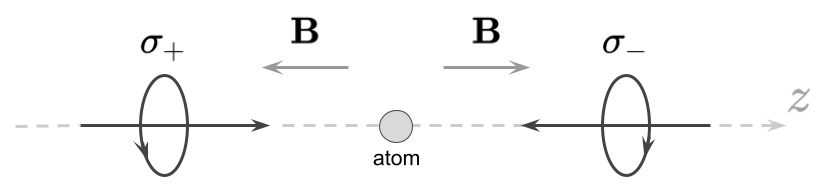
\includegraphics[width=0.7\textwidth]{USPSC-img/1D-MOT.png}
	\vspace{5pt}
	\legend{Simplified one-dimensional MOT composed of two counter-propagating laser beams and a linear magnetic field $ \mathbf{B} = B_0 z \mathbf{e}_z $, where $ B_0 > 0 $. We consider the $ \sigma_{+} $ and $ \sigma_{-} $ beams right-handed and left-handed polarized respectively. \\ Source: Author}
	\label{fig:1D-MOT}
	\vspace{-10pt}
\end{figure}

Disregarding the magnetic field, the transition is properly represented by a degenerate \textit{two-level system} whose energy difference is $ \hbar \omega_0 $. The presence of the magnetic field splits the energy level $ J = 1 $ into three different energy levels $ m_J = 0, \pm 1 $ such that the system turns into a \textit{four-level system} illustrated in figure \ref{fig:1D-MOT-Zeeman-splitting}. This effect is known as \textbf{Zeeman splitting} \cite[Section~7.4]{steck2007quantum}. Essentially, assuming a weak magnetic field\footnote{The quantity $ \mu_B B $, where $ B $ is the magnetic field magnitude, must be much lower than the spin-orbit coupling energy.}, there will be a effective detuning $ \delta_Z^{(m_J)} $ due to the \textbf{anomalous Zeeman effect} so that
\begin{equation}
	\delta_Z^{(m_J)} = - \beta g_{J} m_J z,\ \ \textrm{being}\ \ \beta \equiv \frac{\mu_B B_0}{\hbar},
	\label{eq:Zeeman-shift}
\end{equation}
where $ g_J $ is the \textit{Landé factor} and $ \mu_B $ is the Bohr magneton. The equation (\ref{eq:Zeeman-shift}) is also called \textbf{Zeeman shift}. It is relevant to notice that the detuning depends linearly on the position $ z $ so that $ \delta_Z^{(m_J)} \propto z $.

\begin{figure}[!ht]
	\centering
	\caption{Zeeman splitting in 1D-MOTs}
	\includegraphics[width=0.7\textwidth]{USPSC-img/1D-MOT-Zeeman-splitting.png}
	\vspace{5pt}
	\legend{Zeeman splitting of the transition $ J = 0 \rightarrow J = 1 $ in 1D-MOTs. When $ \mathbf{B} = 0 $ ($\mathbf{B}$ off), the atomic transition $ J = 0 \rightarrow J = 1 $ is described by a \textbf{degenerate two-level system}. However, when $ \mathbf{B} \neq 0 $ ($\mathbf{B}$ on), the same atomic transition is represented by a \textbf{four-level system} in which the excited states are energetically separeted by the Zeeman shift $ \delta_{Z}^{(\pm)} $. The energy scale was not plotted precisely to enhance the visibility.\\ Source: Author}
	\label{fig:1D-MOT-Zeeman-splitting}
\end{figure}

%-----------------------------------
\subsection{Cooling and trapping effect}
\label{sec:cooling-trapping-effect}
%-----------------------------------

Let us consider an arbitrary atom from an atomic cloud in a MOT neglecting interatomic interactions. Although the momentum exchange between atoms and light are quantized, we can evaluate the atom dynamics classically by assuming a mean force $ \mathbf{F}_{MOT} $, which is known as \textbf{semiclassical approach}. It is possible to obtain an analytical expression for $ \mathbf{F}_{MOT} $ under the \textbf{two-level system approximation}, which will be done in the next section \ref{sec:MOT-force}. Without this approximation, we must consider the interplay between optical pumping, photon scattering, Zeeman effect, and Doppler effect in multiple excited states. Therefore, the complexity of the problem will increase considerably. There are only a few articles \cite{prudnikov2015three, choi2008three, PhysRevA.49.4864} that approach this case.

We can be split $ \mathbf{F}_{MOT} $ into two components\footnote{In section \ref{sec:optical-forces}, we deduced both forces for the case of a two-level atom interacting with a single field.}: one exclusively associated with coherent transitions (absorption and \textit{stimulated} emission); and another associated with decoherence decays (absorption and \textit{spontaneous} emission). In weak atom-light coupling, stimulated emission is much less often than spontaneous emission. Therefore, $ \mathbf{F}_{MOT} $ is the \textbf{radiation pressure force}. Essentially, $ \mathbf{F}_{MOT} = (F_{+} - F_{-}) \mathbf{e}_z $, where $ F_{\pm} $ is related to the interaction between atom and the $ \sigma_{\pm} $-beam. Thus, $ F_{\pm} $ depends on the detuning $ \Delta_{\pm} $ so that the lower $ |\Delta_{\pm}| $, the greater $ F_{\pm} $. The detuning $ \Delta_{\pm} $ can be split into three detunings (figure \ref{fig:detuning-1D-MOT}) so that $ \Delta_{\pm} = \delta + \delta_Z^{\pm} + \delta_D^{\pm} $. These detunings are given by
\begin{itemize}
	\item \textit{Laser detuning} $ \delta = \omega - \omega_0 $: associated with the laser frequency $ \omega $ and the energy difference $ \omega_0 $ of the atomic transition. This detuning is the same for all transitions;

	\item \textit{Doppler shift} $ \delta_{D}^{(\pm)} = \mp k v $: associated with the atomic movement (see section \ref{sec:line-broadening-mechanisms});

	\item \textit{Zeeman shift} $ \delta_Z^{(\pm)} \propto \mp z $: associated with the Zeeman splitting. This detuning is given by the equation (\ref{eq:Zeeman-shift}).
\end{itemize}

\begin{figure}[!ht]
	\centering
	\caption{Detuning in 1D-MOT}
	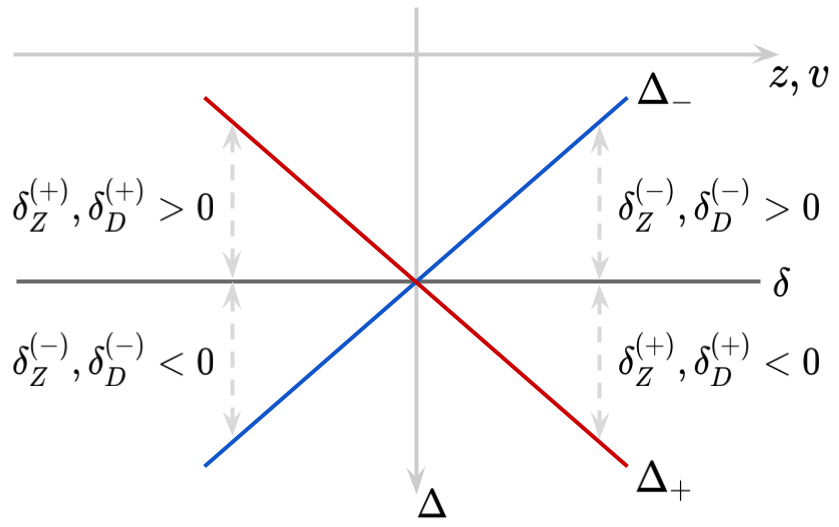
\includegraphics[width=0.55\textwidth]{USPSC-img/1D-MOT-detunings.png}
	\vspace{5pt}
	\legend{Laser detuning, Doppler shift, and Zeeman shift of a 1D-MOT in function of velocity $ v $ and position $ z $ assuming red-detuned laser beams ($ \delta < 0 $). \\ Source: Author}
	\label{fig:detuning-1D-MOT}
	\vspace{-20pt}
\end{figure}

Both Doppler shift and Zeeman shift increase linearly with the atom velocity and atom position respectively. Assuming red-detuned laser beams ($ \delta < 0 $) and $ v > 0 $, the probability of absorbing the $ \sigma_{\pm} $-beam decreases (increase) with $ v $ since $ |\Delta_{\pm}| $ increases (decreases). When $ v < 0 $, the opposite effect occurs. Therefore, the MOT force is opposite to the velocity $ v $ ($ \partial \mathbf{F}_{MOT} / \partial v < 0 $) such as a friction, which is is essentially a \textbf{cooling mechanism} also known as \textbf{Doppler cooling}. The Zeeman shift behaves the same in function of $ z $ such that the MOT force is also opposite to the position ($ \partial \mathbf{F}_{MOT} / \partial z < 0 $), which is essentially a \textbf{trapping mechanism}.

%-----------------------------------
\subsection{MOT Force}
\label{sec:MOT-force}
%-----------------------------------

We shall get deeper into the 1D-MOT analysis by quantifying the MOT force. As mentioned in section \ref{sec:cooling-trapping-effect}, obtain an analytical expression for the MOT forces in the general case is a complicated task. Although, we can obtain such analytical expression under two approximations:
\begin{itemize}
	\item By breaking the four-level system (figure \ref{fig:1D-MOT-Zeeman-splitting}) into three independent two-level systems illustrated in figure \ref{fig:independent-two-level-system}. That is a strong assumption in which the coherence effects between the Zeeman states, such as Raman-like transitions \cite[Section~9.8]{foot2005atomic}, are neglected;

	\item By assuming that the atom density operator $ \hat{\rho}(\mathbf{k}, -\mathbf{k}) $ related to the simultaneous interaction equals the sum of the density operators $ \hat{\rho}_{+}(\mathbf{k}) $ and $ \hat{\rho}_{-}(-\mathbf{k}) $ associated with the individual interactions, which is essentially a superposition ($ \hat{\rho} = \hat{\rho}_{+} + \hat{\rho}_{-} $). This approximation relies on the perturbation theory in first and second-order \cite[Chapter~7]{berman2011principles}. 
\end{itemize}

Both approximations are valid in the regime of weak atom-light coupling so that the total detuning is higher than the power-broadened linewidth.

\begin{figure}[!ht]
	\centering
	\caption{Assumption of independent two-level systems}
	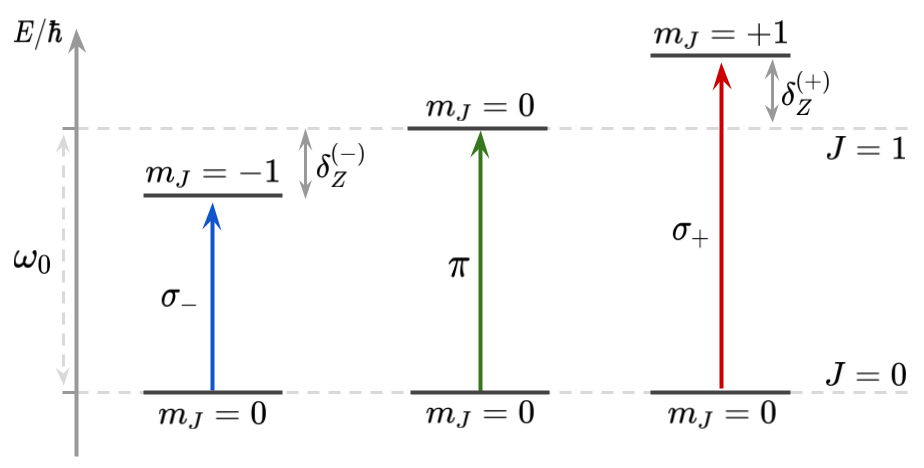
\includegraphics[width=0.6\textwidth]{USPSC-img/Independent-two-level-system.png}
	\legend{Breaking of the four-level system into three independent two-level systems.\\ Source: Author}
	\label{fig:independent-two-level-system}
\end{figure}

Since there are only right-handed and left-handed polarized beams, there will only $ \sigma_{\pm} $-transitions. Therefore, the components $ F_{+} $ and $ F_{-} $ associated with the $ \sigma_{+} $ and $ \sigma_{-} $ transitions respectively are independent radiation pressure forces given by (see section \ref{sec:optical-forces})
\begin{equation}
	F_{\pm}(z, v) = \pm \hbar k \frac{\Gamma}{2} \frac{s_0}{1 + s_0 + 4(\Delta_{\pm} / \Gamma)^2},
	\label{eq:1D-MOT-force-components}
\end{equation}
where $ \Delta_{\pm} = \delta + \delta_{Z}^{(\pm)} + \delta_{D}^{(\pm)} $, $ s_0 $ is the saturation parameter, and $ \Gamma $ is the natural linewidth\footnote{The natural linewidth depends on the energy difference between the states, which is slightly different in each transition. However, this energy difference is much lower than $ \hbar \omega_0 $ such that the natural linewidth is approximately $ \Gamma $.} of the transition $ J = 0 \rightarrow J = 1 $. Assuming low velocities ($ |kv| \ll |\delta| $) and positions close to the magnetic field centre ($ |z| \ll |\delta| $), the MOT force is essentially linear with $ z $ and $ v $ as illustrated in figure \ref{fig:MOT-force}. Hence, we can expand $ F_{MOT} $ about $ z = 0 $ and $ v = 0 $ so that
\begin{equation}
	F_{MOT}(z, v) \simeq F_{MOT}(0, 0) + z \frac{\partial F_{MOT}}{\partial z}(0, 0) + v \frac{\partial F_{MOT}}{\partial v}(0, 0),
	\label{eq:MOT-force-Taylor-expansion}
\end{equation}

\begin{figure}[!ht]
	\centering
	\caption{MOT force}
	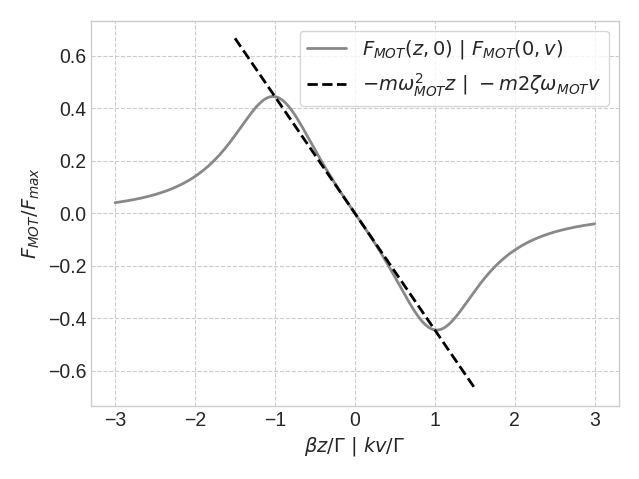
\includegraphics[width=0.5\textwidth]{USPSC-img/MOT_force.png}
	\legend{Plotting of the MOT force $ F_{MOT} $ for $ v = 0 $ ($ z = 0 $) in function of $ \beta z / \Gamma $ ($ k v / \Gamma $) considering the transition $ {}^{1}S_0 \rightarrow {}^{1}P_1 $ of the $ {}^{88}Sr $ for $ \delta = - \Gamma $ and $ s_0 = 1 $. The dashed line in the graph is the MOT force assuming $ |\beta z| \ll |\delta| $ ($ |kv| \ll |\delta| $).\\ Source: Author}
	\label{fig:MOT-force}
\end{figure}

Rearranging the terms of equation (\ref{eq:MOT-force-Taylor-expansion}), we obtain
\begin{gather}
	\frac{d^2 z}{dt^2} + 2\zeta \omega_{MOT} \frac{d z}{d t} + \omega_{MOT}^2 z = 0,
	\label{eq:damped-harmonic-oscillation-1D-MOT}
	\\
	\omega_{MOT}^2 \equiv - \frac{1}{m} \frac{8 \hbar k \beta g_J s_0 (\delta / \Gamma)}{[1 + s_0 + 4(\delta / \Gamma)^2]^2},\ \ \textrm{and}\ \ \zeta \equiv \frac{k}{2\beta g_J} \omega_{MOT},
	\label{eq:constants-equation-of-motion-1D-MOT}
\end{gather}
where $ m $ is the atomic mass. The quantity $ \omega_{MOT} $ has unit of frequency and $ \zeta $ is a dimensionless quantity. Also, $ \omega_{MOT}^2 $ is a positive real value since we are assuming red-detuned lasers, which means $ \delta < 0 $ in equation \ref{eq:constants-equation-of-motion-1D-MOT}. The equation of motion (\ref{eq:damped-harmonic-oscillation-1D-MOT}) describes a \textit{damped harmonic oscillation} of which $ \omega_{MOT} $ is the \textit{undamped frequency} and $ \zeta $ is the \textit{damping ratio}. Therefore, the atom is trapped by the restoring force $ - m \omega_{MOT}^2 z $, being limited to move in a restricted region (\textbf{trapping mechanism}). Furthermore, the atom loses energy due to the damping $ 2 \zeta \omega_{MOT} v $ can be understood as a \textbf{cooling mechanism}.
